\documentclass{beamer}
\usetheme{Boadilla}
\usepackage{tikz}
\usepackage{graphicx}
\usepackage{amsmath}
\usetikzlibrary{shapes.geometric,arrows, positioning, fit}




\title{Weekly Presentation}
\subtitle{Week 41}
\author{}
\institute{Luleå University of Technology}
\date{\today}



\begin{document}
\begin{frame}
    \titlepage
\end{frame}

\begin{frame}
    \frametitle{Overview}
    \tableofcontents
\end{frame}

%%%%%%%%%%%% Add new frames below this line %%%%%%%%%
\section{Status update}
\begin{frame}
    \subsection{Time plan}
    \frametitle{Overall timetable}
    \begin{table}
        \begin{tabular}{| l | c | c | c | c }
            
            Sep & Oct & Nov & Dec \\
            \hline \hline
            Concept generation & Evaluation & Evaluation &  \\ 
            \hline
            Theory & Prototyping & Evaluation & Finishing up \\
            \hline
            Simulation & Evaluation & Evaluation & \\
            \hline
            Prototyping & Final Design & Evaluation &  \\
            \hline
 
        \end{tabular}
    \end{table}    
\end{frame}


\begin{frame}
    \frametitle{Time plan for September}
    \begin{table}
        \begin{tabular}{l | c | c | c | c }
        Subproject & Week 1 & Week 2 & Week 3 & Week 4 \\
        \hline \hline
            Arrowhead & Reading& Setup & API & Prototyping\\
            Movable base & Reading& Modeling & Simulation & Implementation\\
            Arm and grip  & Reading & Kinematics & Simulation& Prototyping\\
            Object detection & Reading & Testing & Prototyping & Evaluation\\
        \end{tabular}
    \end{table}
\end{frame}
\tikzstyle{Process} = [rectangle, draw]

\tikzstyle{Start} = [draw, rectangle, rounded corners] 

\tikzstyle{Data} = [draw,trapezium,trapezium left angle=70,trapezium right angle=-70]

\tikzstyle{Decision} = [diamond, draw] 
\begin{frame}
    \subsection{Report workflow}
    \frametitle{Report workflow}
    
\centering
\resizebox{7.0cm}{!}{
\begin{tikzpicture}
    [align=center, auto]
    \node [Start] (start) {\textbf{CHAPTER\_descriptive\_filename.tex}};
    \node [Process, below= of start] (push) {Push to \textbf{/sections}};
    \node [Decision, below= of push] (finished) {Finished?};
    \node [Data, below= of finished] (write) {Write on section}; 
    \node [Process, below= of write] (commit) {Commit};

    \node [Process, right= of finished, xshift=5em] (branch) {New branch \\ \textbf{REVIEW\_chapter}};
    \node [Data, below= of branch] (paste) {Paste section in \\ \textbf{/chapters/chapter.tex}};
    \node [Process, below= of paste] (pushb) {Push new branch};
    \node [Data, below=of pushb] (PR) {PR against \textbf{report-unsafe}};
    \node [Start, below= of PR] (review) {Wait for review};
    
    



    \coordinate [left= of push] (lrpush);
    \coordinate [left= of write] (lrwrite);
    \coordinate [left= of commit] (lrcommit);
    \coordinate [left= of finished] (lrfinished);
    \coordinate [right= of PR] (crPR);
    \coordinate [below= of crPR] (crreview);
    



    \draw [->] (commit) -- (lrcommit) -| (lrpush) -- (push);

    \draw [->] (start) -- (push);

    \draw [->] (push) -- (finished) -- node[midway, fill=white] {No} (write) -- (commit);

    \draw [->] (finished) -- node[midway, fill=white] {Yes} (branch);

    \draw [->] (branch) -- (paste) -- (pushb) -- (PR)  -- (review);

    \draw [->] (review) -| (crreview) -- node[midway, xshift=2.2em, yshift=-0.5em, fill=white] {Fix} (crPR) -- (PR);
    
    
\end{tikzpicture}
}
\begin{center}
    \small https://github.com/kottz/D7039E/tree/report-unsafe
\end{center}

\end{frame}

\begin{frame}
    \frametitle{Finished}
    \begin{figure}
        \resizebox{7.0cm}{!}{
        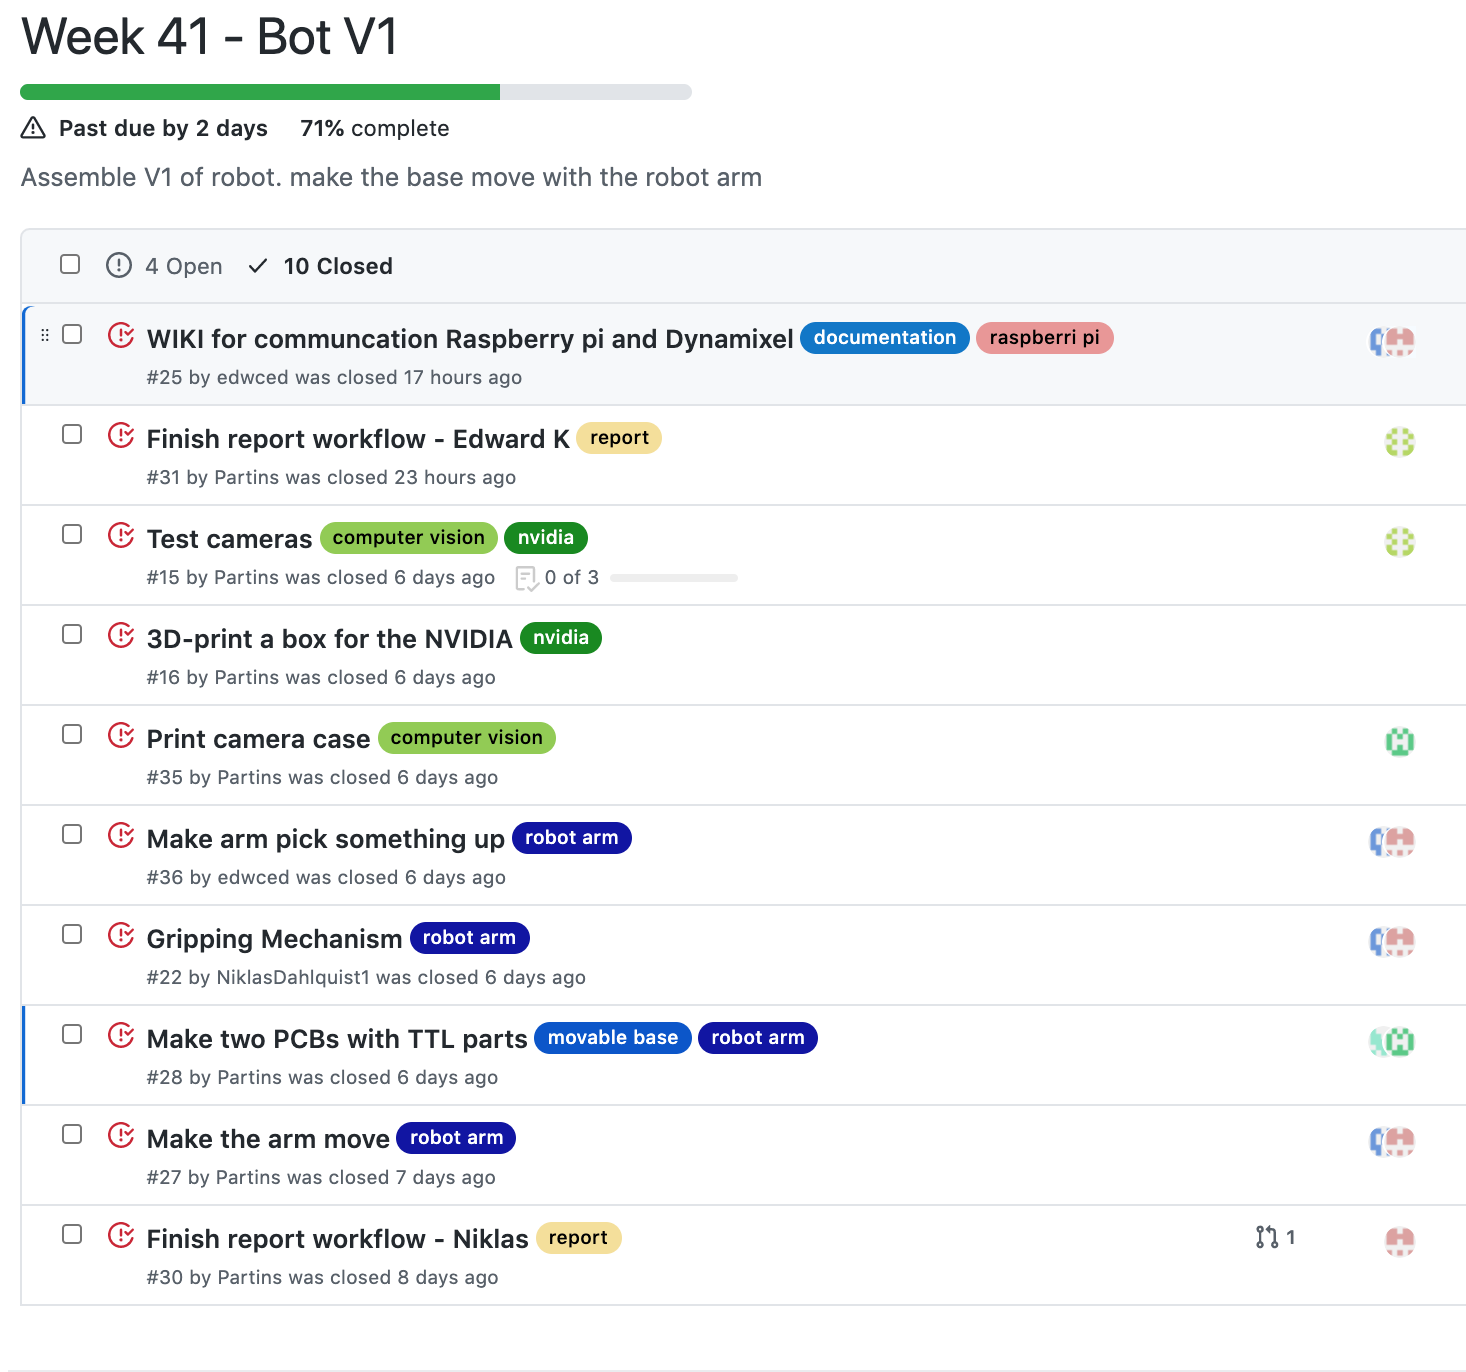
\includegraphics[width=\textwidth]{frames/img/milestone_week41_finished.png}
        }
    \end{figure}
\end{frame}

\begin{frame}
    \frametitle{Unfinished}
    \begin{figure}
        \resizebox{7.0cm}{!}{
        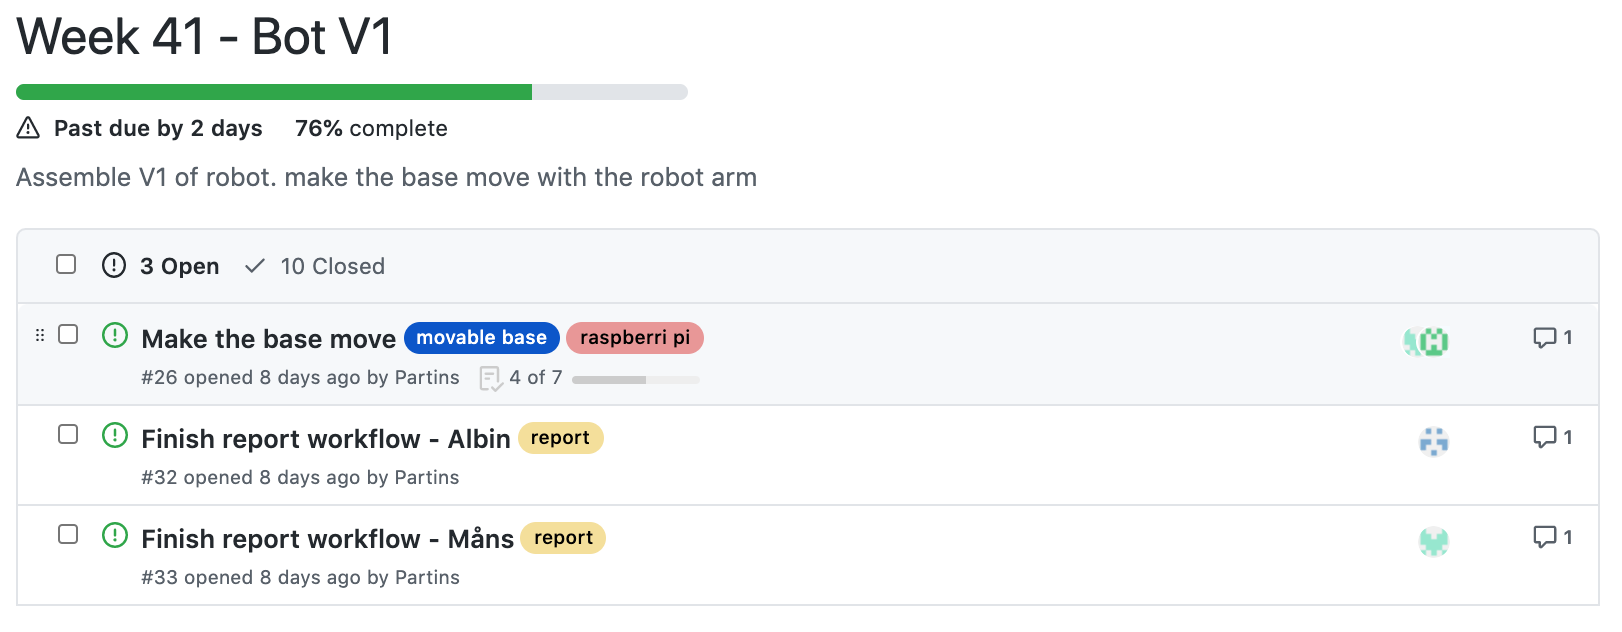
\includegraphics[width=\textwidth]{frames/img/milestone_week41_unfinished.png}
        }
    \end{figure}
\end{frame}

\begin{frame}
    \frametitle{Weekly plan}
    \begin{figure}
        \resizebox{7.0cm}{!}{
        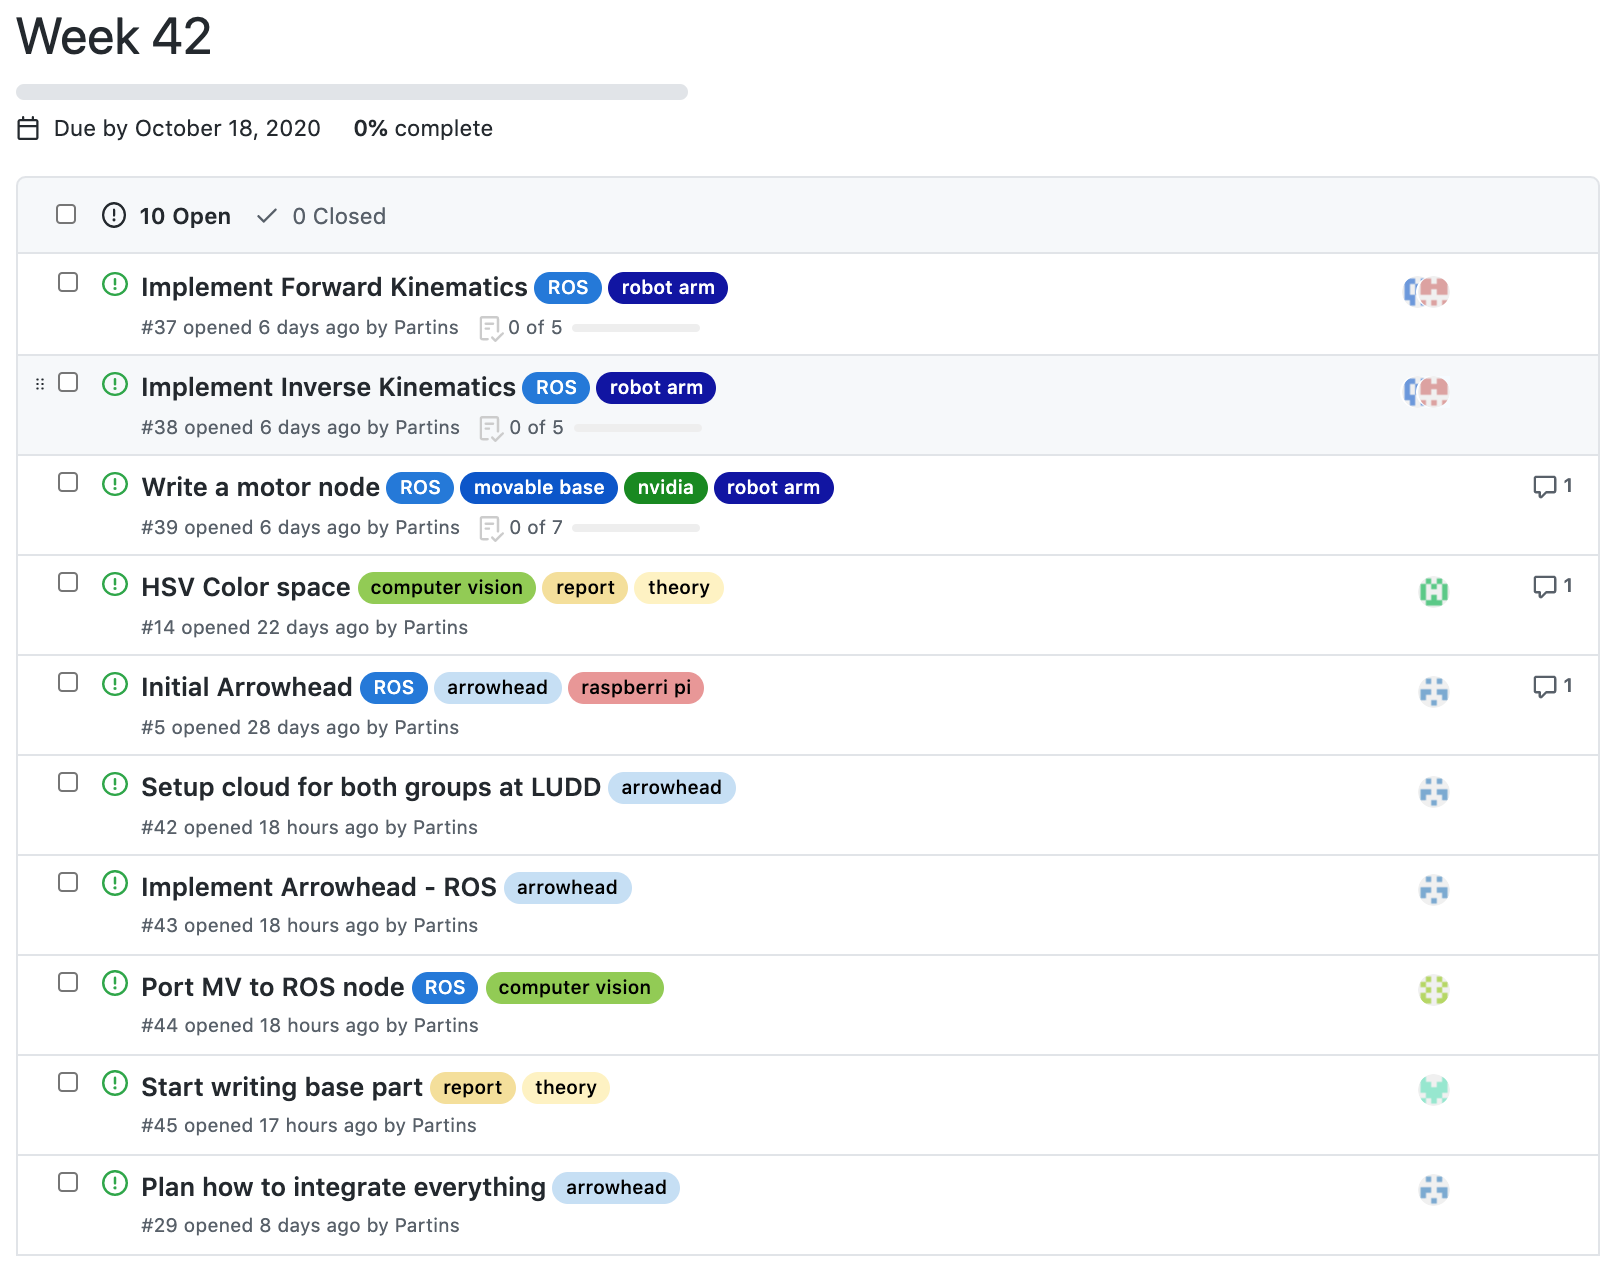
\includegraphics[width=\textwidth]{frames/img/milestone_week42.png}
        }
    \end{figure}
\end{frame}

\section{Positioning - Arrowhead}

\begin{frame}
    \frametitle{Positioning - Arrowhead}
    \centering
    
\resizebox{9.0cm}{!}{

\begin{tikzpicture}
    [align=center, node distance = 2em,  auto]

    %% Robot
    \node [Start] (start) {Start};
    \node [Data, below= of start] (findqr) {Find and read QR};
    \node [Data, below= of findqr] (report) {Report to \\ Arrowhead};
    \node [Data, below= of report] (getgood) {Wait for instruction \\from Arrwohead};
    \node [Process, below= of getgood] (follow) {Work on goal};
    \node [Data, left= of report, yshift=-2em] (status) {Report status \\ to Arrowhead};

    %% Arrowhead
    \node [Process, right= of report, xshift=10em] (arrowstart) {Decide on goal \\ for robot};
    \node [Process, below= of arrowstart, yshift=-0.5em] (certify) {Certify robot};


    %% Draw
    \draw (start) -- (findqr) -- (report) -- (getgood) -- (follow);
    \draw [->] (follow) -| (status) |- (findqr);

    
    \draw [->, dashed] (report) -- node[midway, fill=white, yshift=-1.5em] {Status/ \\ Position} (arrowstart);
    \draw [->] (arrowstart) -- (certify);
    \draw [->, dashed] (certify) -- (getgood);

\end{tikzpicture}
}
\end{frame}

\section{Robot arm movement}
\begin{frame}
    \centering
    \Huge Robot Arm
    
\end{frame}



%%%%%%%%%%%% Add new frames above this line %%%%%%%%%


\begin{frame}
    \begin{center}
        \Huge Questions?
    \end{center}
\end{frame}





\end{document}